% \subsection{Pré-processamento de Textos}



O pré-processamento é a etapa que difere o processo de Mineração de Textos do processo de Mineração de Dados. Uma vez que os texto estão em formato inerentemente não estruturado, o problema se resume em adequá-los para uma representação estruturada, concisa e manipulável por algoritmos de Aprendizado de Máquina, além de limpeza e redução de termos.


% \subsection*{Extração de texto}

Os documentos da coleção frequentemente encontram-se em diferentes formatos dado a diversidade de \textit{softwares} para edição e publicação de conteúdos digitais. Assim, o processo se inicia com a extração do texto em formato plano (puro), em seguida transformado em um formato mais adequado. 
%
%
% \subsection*{Remoção de atributos }
% 
Os dados textuais têm como características serem esparsos e apresentar alta dimensionalidade. Por exemplo, uma coleção de documentos frequentemente contém milhares de palavras, ao passo que um documento específico irá conter uma pequena parcela dessa diversidade, em torno de algumas centenas. Essas características, por consequência, exigem que os dados originais sejam reduzidos, porém preservando as caraterísticas mínimas para os algoritmos utilizados a seguir.


\subsection*{Remoção de \textit{Stop Words}}

Considerando a alta dimensionalidade dos textos, os termos menos significativos devem ser removidos.  \textit{Stop words} são palavras pouco relevantes que não contribuem para a distinção do texto em tópicos ou categorias podem ser removidas, como artigos, preposições, pronomes, verbos de estado\footnote{Apresentam uma situação inativa, onde o verbo não expressa uma alteração, mas apenas uma propriedade ou condição dos envolvidos.}. Trata-se também como \textit{stop words} as palavras de uso muito frequente dentro de um determinado domínio não são capazes de discriminar documentos e também não devem fazer parte dos atributos. A eliminação das \textit{stop words} é feita com base em um conjunto de palavras conhecido como \textit{stoplist}.








\subsection*{Corte por Frequências}

Outra forma utilizada para seleção de termos é avaliar a importância de cada termo por meio de medidas estatísticas, como o TF (\textit{term frequency}) e DF (document frequency). O método proposto em~\cite{Luhn1958} é uma técnica baseada na Lei de Zipf~\cite{zipf1932} também conhecida como Princípio do Menor Esforço, em que computando-se a frequência das palavras de um texto, e criando-se seu histograma em ordem decrescente, observa-se a chamada Curva de Zipf, na qual o $k$-ésimo termo mais comum ocorre com frequência inversamente proporcional a $k$. Os termos com alta frequência são considerados pouco relevantes por serem comuns à grande maioria dos documentos, enquanto termos mais raros não possuem caráter discriminatório suficiente. Assim, é possível estabelecer pontos de corte nos extremos da curva, a fim de manter termos com frequência intermediária, os quais são os mais representativos do documento~\cite{Maracini2010}. Na Figura~\ref{fig:luhn} é ilustrada a distribuição do termos mais relevantes em um documento e a curva de Zipf com dois cortes nas extremidades.


  \begin{figure}[!h]
	  \centering
	  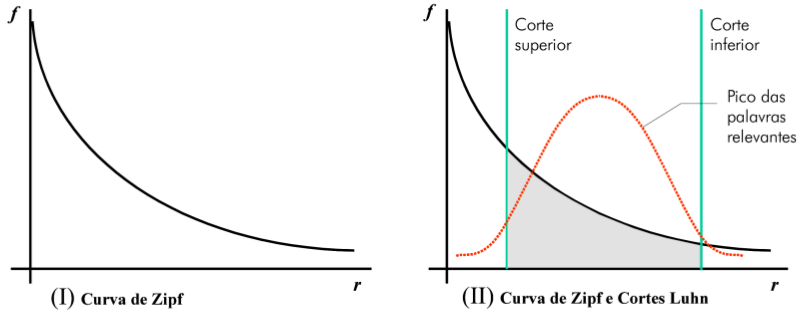
\includegraphics[width=0.85\textwidth]{conteudo/capitulos/figs/luhn2.png}
	  \caption{A curva de Zipf e os cortes de Luhn~\cite{Soares2008}.}
	  \label{fig:luhn}
  \end{figure}




% \subsection*{Transformação de Atributos}
\subsection*{\textit{Stemming}}


% As palavras não removidas na seleção de termos passam ainda por um processo conhecido como \textit{stemming}.
A radicalização ou \textit{stemming} é a redução das variações de uma palavra ao seu provável radical ou stem a fim de associar palavras semelhantes e diminuir a dimensionalidade da representação do texto.
Nesse processo, as palavras são reduzidas ao seu provável radical ou \textit{stem}, a fim de se associar palavras semelhantes e diminuir a dimensionalidade da representação do texto. Por exemplo, os termos ``\textit{agenda}'', ``\textit{agendamento}'' e ``\textit{agendar}'' dever ser todas reduzidas ao seu radical em comum ``\textit{agend}''. Com isso, a dimensionalidade é diminuída ainda mais e tem-se um texto formado apenas por morfemas\footnote{Em Morfologia, um morfema é a menor unidade capaz de expressar significado.} com maior significância.  
% 
% O algoritmo de Porter, é amplamente utilizado em sistemas que processam texto na língua inglesa e frequentemente eficaz na remoção de sufixos. 
% proposto por Martin Porter em 1980 
% Por outro lado, insuficiente para outros idiomas, uma vez que, seu mecanismo é altamente dependente do idioma inglês.
%

Em geral, algoritmos de \textit{stemming} dependem do uso adequado da ortografia da língua em questão, inclusive com acentuação correta, sendo em alguns casos recomendado o uso de corretores automáticos na fase de pré-processamento. A língua portuguesa particularmente apresenta algumas dificuldades, na elaboração de algoritmos de \textit{stemming}, das quais destacam-se o número elevado exceções e homófagos; palavras com mudanças no radical morfológico; nomes próprios que não podem ser radicalizados e frequência de termos estrangeiros.  É possível identificar alguns erros apresentados pelos algoritmos de \textit{stemming} que reduzem a qualidade os resultados da Mineração de Texto, como \textit{oversteamming:} quando o algoritmo remove parte do radical e \textit{understeamming:} quando o algoritmo não remove totalmente o sufixo.

O uso de \textit{stemming}, de uma maneira geral, pode trazer algumas desvantagens das como a perda de contexto, pois palavras com sentidos diferentes podem resultar no mesmo radical, aumentando assim a quantidade de homônimos e a perca da precisão que diminui a variedade de palavras causando certa perda de informação. Contudo, eventuais perdas de informação por \textit{stemming} não causam grandes impactos sobre a eficiência de algoritmos de text mining e seu uso se justifica pela redução da dimensionalidade da base de textos.



